\let\cleardoublepage\clearpage
%% ----------------------------------------------------------------
%% Introduction.tex
%% ---------------------------------------------------------------- 

\chapter{Specification} \label{Chapter:Specification}
Our quadcopter relies on collecting data from a Grove IMU 9DOF v2.0 unit. This is based on the MPU-9250 chip, incorporates a digital 3-axis accelerometer, gyroscope and magnetometer, and offers I2C or SPI interface options. We decided to use the I2C protocol to make use of the faster speed of 400 Hz.  The PID control and pwm motor interface all takes place on a Seeeduino (Arduino clone), so it makes sense that this microcontroller also reads the sensor values. Because of previous experience our initial plans were to program the microcontroller in pure C, and use AVRdude to flash programs to the ATmega328p chip. However, upon further research I discovered that it’s possible to code libraries in C or C++, and simply call them in the Arduino IDE. This allowed us to make use of a wider range of already available libraries for the Arduino platform, but still develop our own code in a lower level language we had experience coding in.

The flight controller program loop needs to operate at a frequency of at least 50 Hz (20ms) to provide adequate control over the drone. Therefore, the aim was to read sensors at a rate of 100 Hz. 

\begin{figure}[H]
	\centering
	\subfigure{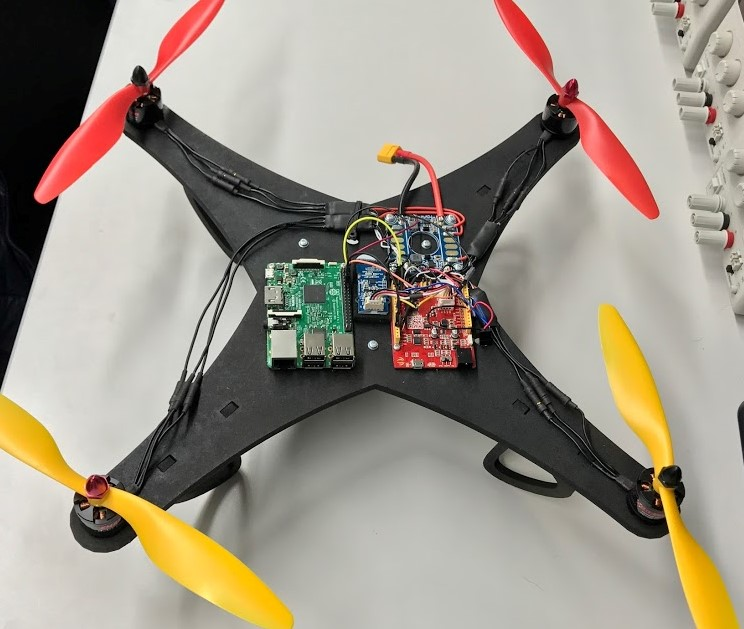
\includegraphics[width=13cm]{figures/drone}}
	\caption{Our final constructed drone.The IMU sits directly in the centre of the frame and is mounted on foam to dampen vibrations from the motors.}
	\label{fig:drone}
	\hfill
\end{figure}